\chapter{Preparation of data}
\section{The "Cut"}
Firstly, let's take stock of the datasets at our disposal. We have four different datasets: results.csv (1872-present), goalscorers.csv (1916-present), shootouts.csv (1967-present), and rankings.csv (1992-present), along with fifa\_country\_list.csv.\\

When embarking on a project involving multiple datasets, it is crucial to start with proper data preparation. The key to any machine learning task lies in thorough data preparation.\\

In our case, the initial step involves a "cut" based on dates. The idea is straightforward: choose a date and retain all data prior to the selected date. Analyzing the project's datasets reveals a natural choice as we encounter four distinct dates: 1872, 1916, 1967, and 1992. These dates exhibit a considerable chronological gap.\\

Selecting the date for data filtering, however, proves to be more intricate. Several possibilities exist, and none are inherently incorrect. Beginning with the most obvious, considering 1872 is unnecessary. Football's origins at that time were more of a recreational activity for sailors than the internationally recognized professional sport we know today. Moreover, the involvement was primarily limited to British countries, making it incompatible with the project's goal of predicting a modern international football event.\\

Considering the first organized World Cup in 1930 could be a valid option. This aligns with the emergence of international football tournaments, including the World Cup, signifying a more developed global football scenario. However, this choice propels us too far ahead in time, where football significantly differed in terms of technology, rules, and World Cup format mutations.\\

The sentiment turns nostalgic when considering 1950 onwards. For many ardent football enthusiasts, sidestepping the football scene from 1950 onwards is inconceivable. The emergence of football stars such (Di Stefano,Pelé, Yashin, Eusebio), dynasties like Real Madrid and AC Milan, and prestigious trophies like the European Cup and Ballon d'Or make this period pivotal. Unfortunately, our model does not focus on this era.\\

After delineating reasons for not considering earlier dates that hold significance in football history, let's settle on the final date. We opted for a "cut" in 1996. This choice is influenced by the contemporary World Cup format with a total of 32 teams and the year 1996 marks the commencement of playoffs for the 1998 World Cup. This World Cup is of particular interest as it introduces the 32-team format for the first time. Mirroring what we aim to predict: the Qatar 2022 World Cup. By ending just before the Qatar World Cup, we ensure our predictions are unbiased.\\

Regulatory considerations play a role, too, as the rules in 1996 align closely with today's standards. Choosing an earlier date might introduce variations such as matches without offside rules, goalkeepers handling back passes from teammates'feet, and restrictions on substitutions.\\

To conclude this section, selecting 1996 ensures that all datasets are available, as they all provide data from 1992 onwards. This eliminates the need for additional internet searches to fill in missing data, especially relying on the intricate FIFA rankings, which would otherwise be challenging to recreate independently.\\
\newpage
\section{Fixes on the list of countries}

Choosing data from 1996 for analysis has significant advantages, especially regarding how countries are named. This approach avoids issues related to disappeared political entities, like the Soviet Union, and makes it easier to compare data among countries that have undergone changes in their names. By focusing on this period, we consider the disappearance of outdated entities, such as Yugoslavia, and the recognition of new states. This allows for analysis in a context where international relations have become more stable, while avoiding ambiguities related to naming countries during periods of political transition. Thus, analyzing data from 1996 provides a strong foundation for understanding the current political realities of countries while maintaining consistency in their national identification.\\

Our dataset could contain several countries with different or outdated nomenclatures; therefore, we had to organize the dataset.\\
\begin{figure}[h]
  \centering
  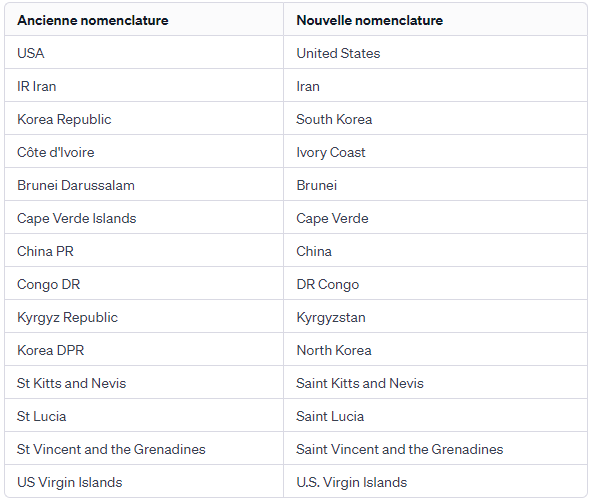
\includegraphics[width=0.8\linewidth]{countries.png}
  \caption{Mapping of Former and Updated Nomenclature in FIFA Rankings}
\end{figure}\\

\newpage
\section{Resampling}
Once the data has been filtered, we proceed to organize the new datasets. The initial step involves renaming "rank\_date" to "date" for uniform attributes. In this ongoing effort, we proceed to create a dataset named "daily\_ranking," which is essentially a version of the filtered rankings dataset but tailored for each unique date present in the filtered match results. This approach allows us to have a dataset that provides the ranking as of the date for each played match.
\section{Merging Data}
In this data merging step, the goal is to integrate information related to match results with daily rankings. Several operations are conducted for this purpose.
Firstly, a redundant column named 'country\_full' is dropped from the daily rankings DataFrame (daily\_ranking). This elimination is necessary to avoid conflicts during the subsequent merging of data. Additionally, the DataFrame's index is reset to convert the 'date' and 'country\_full' columns from index to regular columns, making it easier for future data manipulation.
The first merge is performed with the filtered match results DataFrame (results\_filtered). Data for home teams is merged using the 'home\_team' and 'date' columns from the results DataFrame and the 'country\_full' and 'date' columns from the modified daily rankings DataFrame. This operation employs the pd.merge method with the how='left' parameter, ensuring that all rows from the results DataFrame are included, while only the corresponding rows from the rankings DataFrame are added.
Post-merge, resulting columns are renamed to clearly indicate that they represent characteristics of the home team; for instance, 'rank' becomes 'home\_rank'. This step aims to enhance data comprehensibility and avoid potential confusion during subsequent analysis.
Next, a second merge is executed with the daily rankings DataFrame to incorporate features of the away teams. Similarly, the 'away\_team' and 'date' columns from the results DataFrame are matched with the 'country\_full' and 'date' columns from the rankings DataFrame, again using the pd.merge method with how='left'.
Once more, resulting columns are renamed, this time to indicate that they represent features of the away team; for example, 'rank' becomes 'away\_rank'.
In summary, this data merging step creates a new DataFrame called "rera" that seamlessly integrates relevant information for football match analysis, clearly distinguishing features of home and away teams. This process ensures data consistency and facilitates interpretation during subsequent analysis steps.

